\section{Browsing}
In this section, I selected my venue based on the h-index relevance metric. The 2024 volume 25, issue 5 of the "Briefings in Bioinformatics" \ref{BriB} with an h-index of 115 was my venue choice for this exercise.

\begin{figure}[h]
    \centering
    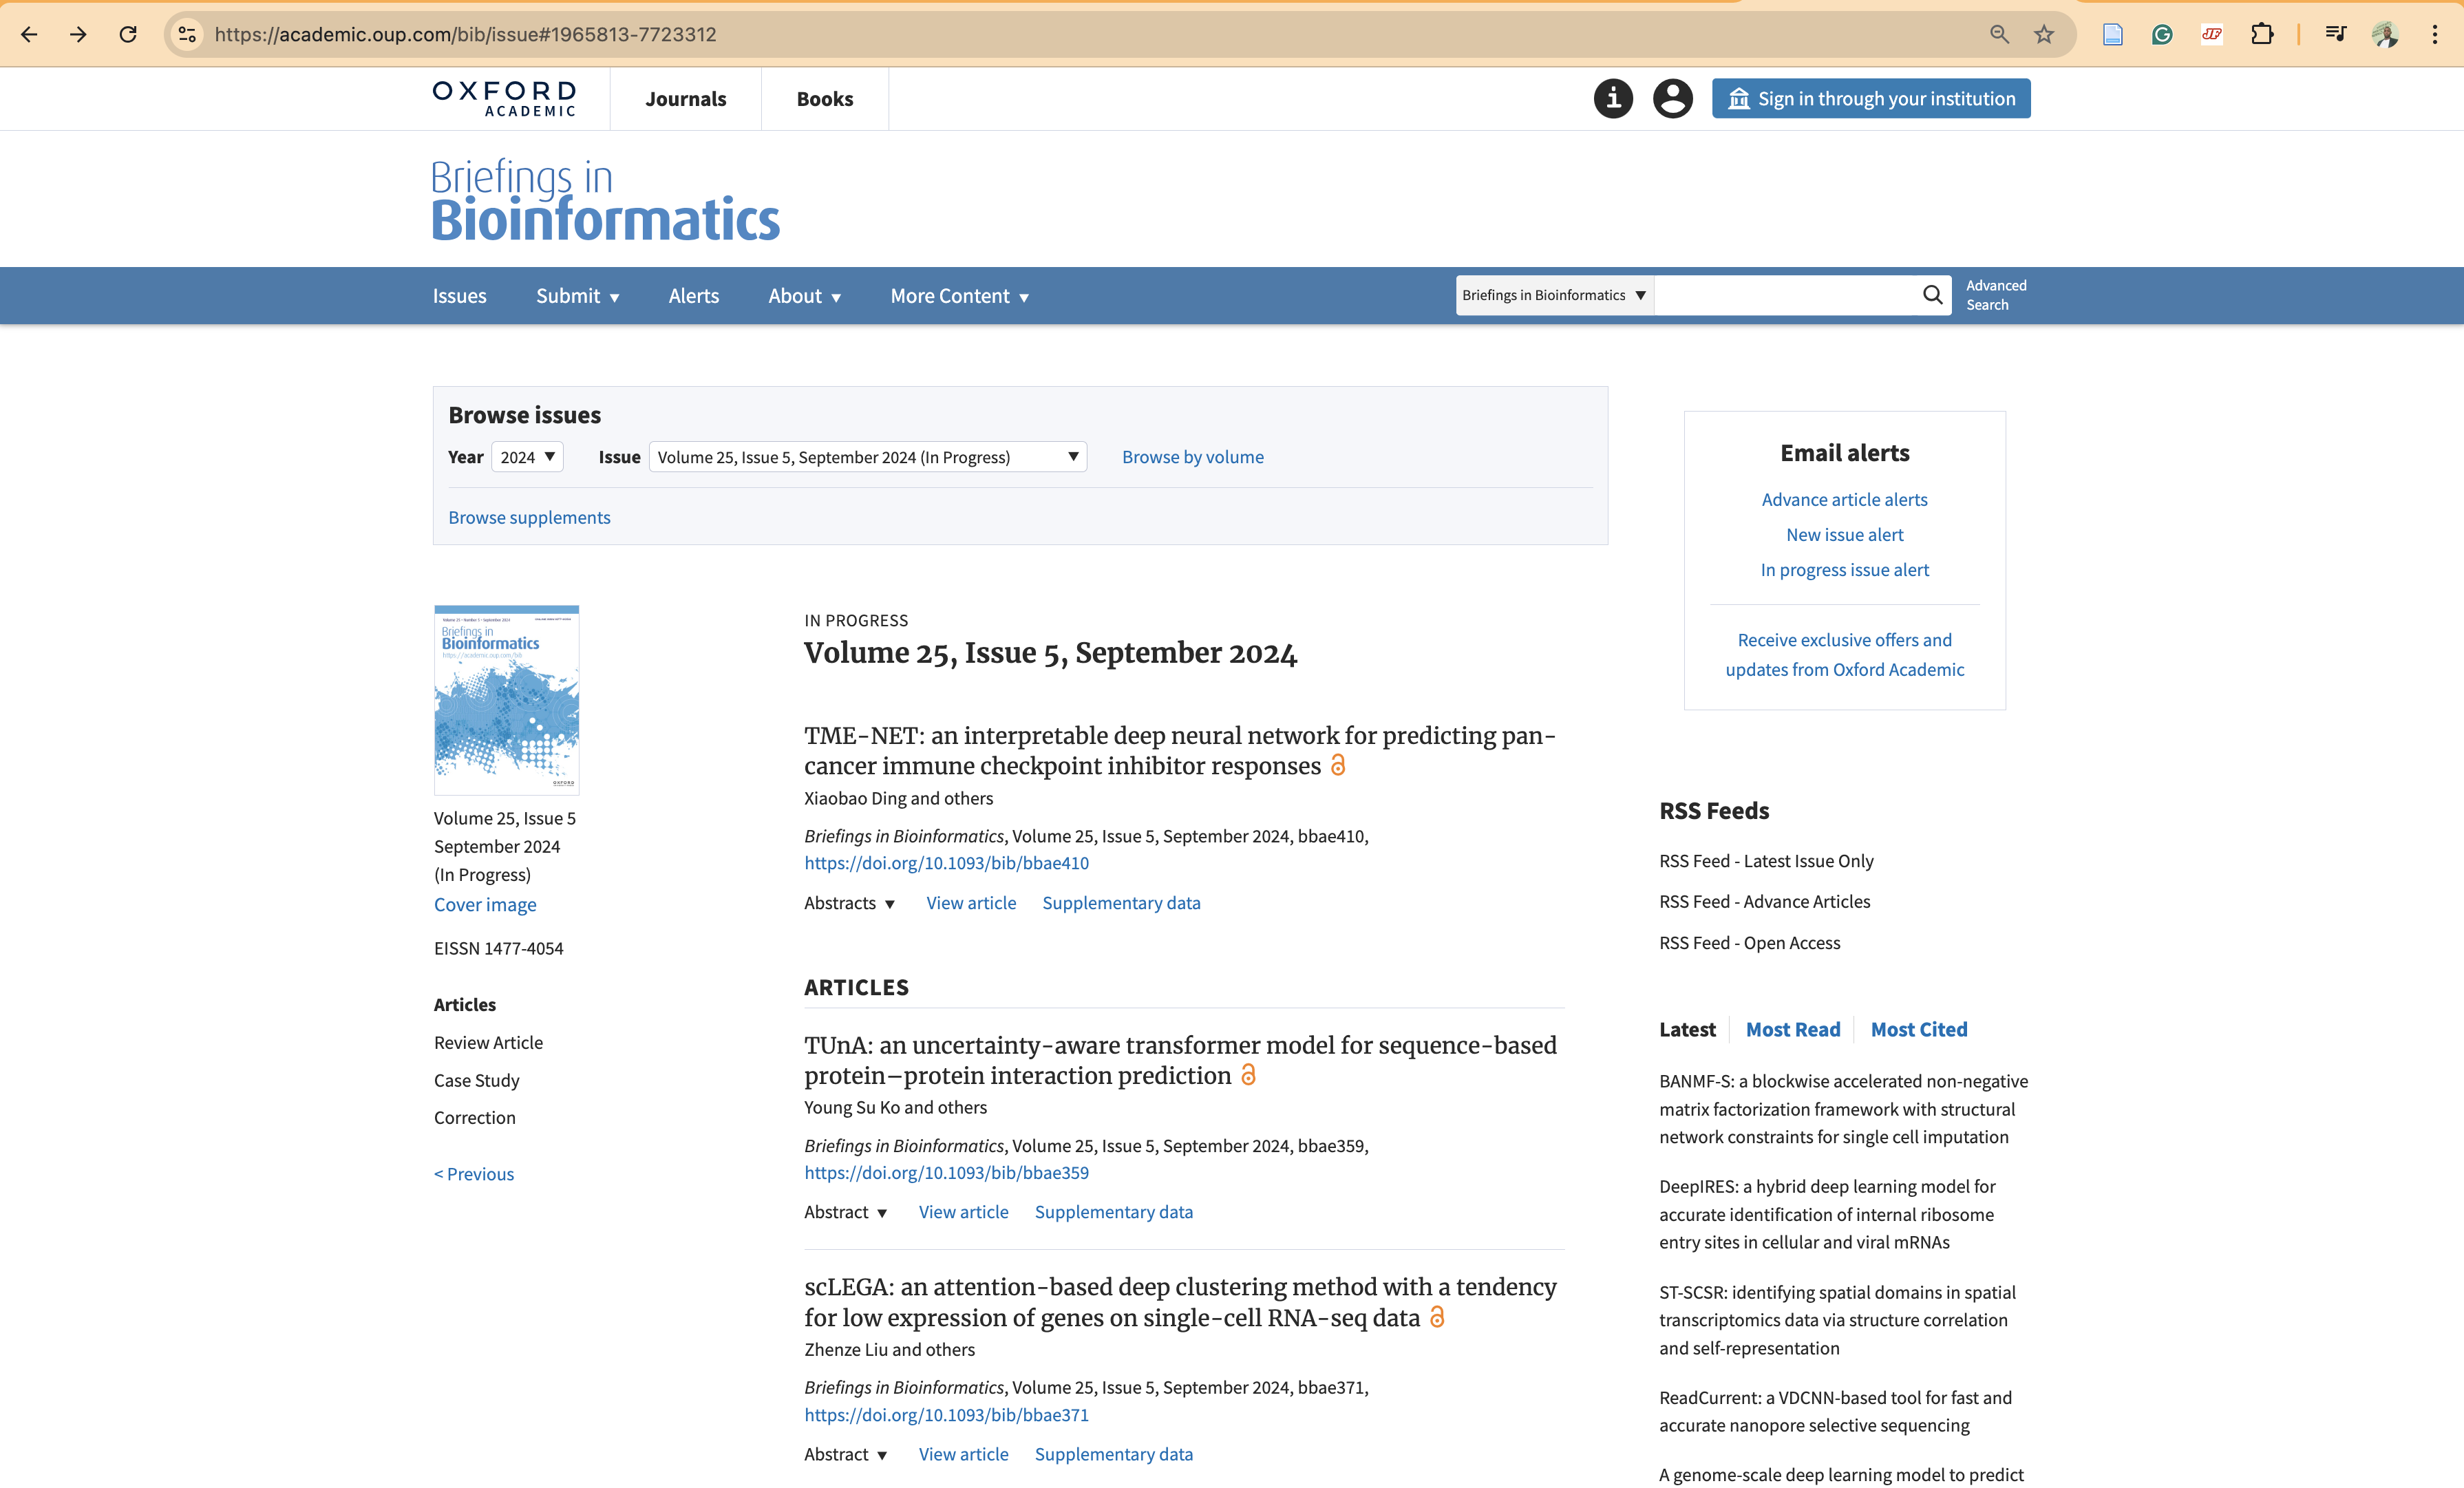
\includegraphics[width=0.8\textwidth]{images/J2Venue.png} 
    \caption{Briefings in Bioinformatics issue content page.}
    \label{BriB} 
\end{figure}

The browsing process was somewhat challenging at first, as I fought with zoning exclusively into browsing mode and not deviating into scan mode. This happened for the first few papers, but as I proceeded with the consciousness of the differentiating fine line between the two processes, I gradually built the discipline to zone into the process at hand wholly.

\subsection{Critical Reading Exercise}
\subsubsection{CAPE}
\begin{itemize}
    \item Attention mechanism was used for promoter evolution
    \item The Dataset used is a simulated one
    \item Author employed the use of Chaos Game Representation to handle the data supply into the model.
    \item The model emphasizes the applicability of transfer learning, with performance demonstration of about $8\%$ better than existing models.
    \item The author proved sufficiently that their model is effective in drug production, synthetic biology-related promoter elucidation, and other closely related prokaryotic promoter-associated functions.
\end{itemize}


\subsubsection{TUnA}
\begin{itemize}
    \item The paper introduces a deep learning model for the prediction of protein-to-protein interactions (PPI)
    \item The architecture employed the use of ESM-2 embeddings for the protein sequence input
    \item The authors incorporated dual transformer encoding - one is designed to handle intra-protein features extraction, while the other deals with the inter-protein capturing
    \item In a bid to reduce false positives and aid the identification of more reliable predictions, TUnA featured uncertainty awareness into its PPI prediction
    \item The dataset used for this research was filtered for physical low sequence similarity across species instead of simulating it, fusing some more level of practicality in the author's submission
    \item The model established its potency with superior computational efficiency, higher accuracies and better calibration in comparison with existing models.
\end{itemize}